\section{Traversal: DFS and BFS}

Traversing a graph means visiting its nodes in some order.
To do that, we need to store the nodes we discover in a container
so that we remember to explore them later.
In this section, we will introduce the different containers
we will use for that,
then what kind of behavior they induce in the traversal.

\subsection{Stacks and queues}

Stacks and queues are the containers we will use here.
They are very similar in nature, and they are both special cases of
\emph{deques}, double-ended queues, but they will make a huge difference
in the order of exploration.

Deques are lists that allow insertion, access and deletion
of elements on both ends, in constant time.
We will not worry about the implementation here.

A \emph{stack} only allows insertion, acess and deletion
at the back of the list.
We can view it as a stack of pancakes: you can only add or remove a pancake
at the top of the pile.
It follows the \emph{LIFO} (last-in-first-out) principle:
the last element that is inserted is the first to be processed.
\begin{center}
    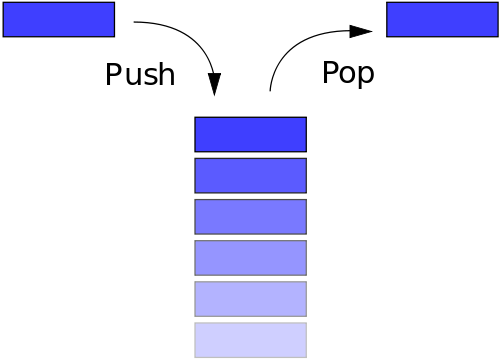
\includegraphics[width=0.3\textwidth]{img/stack}
\end{center}

A \emph{queue}, on the other hand allows insertion only at the back,
while acess and deletion only happen at the front.
We can view it as a queue at the checkout in a store.
It follows the \emph{FIFO} (first-in-first-out) principle:
the elements are processed in the same order that they were inserted.
\begin{center}
    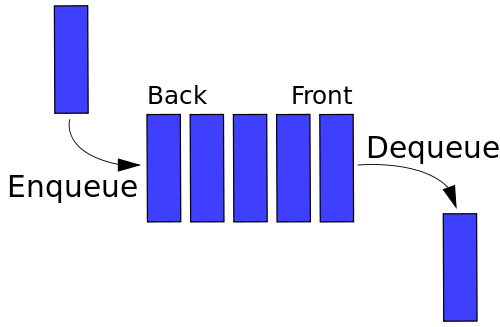
\includegraphics[width=0.3\textwidth]{img/queue}
\end{center}

The corresponding function members are \texttt{.push()} for insertion,
\texttt{.pop()} for deletion and for acess, stacks have \texttt{.top()}
and queues have \texttt{.front()}.

\subsection{Depth-first search}

When traversing a graph, the same procedure happens over and over again:
\begin{itemize}
    \item choose a node;
    \item check that it has not been visited before;
    \item process the node;
    \item add its neighbours to the waiting list.
\end{itemize}

At the beginning, we add the starting point to the waiting list,
then we execute that procedure until the waiting list is empty.

If the graph is connected, it means we have traversed it entirely.
Otherwise, it means we have traversed one \emph{connected component}
of the graph, and we have to choose a new starting point.

\emph{Depth-first search}, or \emph{DFS}, uses a stack as waiting list.
The consequence is that as soon as a new node is discovered, it will be
explored, so depth-first search will progress quickly through the graph,
going in \emph{depth}
instead of exploring its most direct neighbourhood first.

The diagram below shows the order in which nodes are visited,
taking the example of a tree:
\begin{center}
    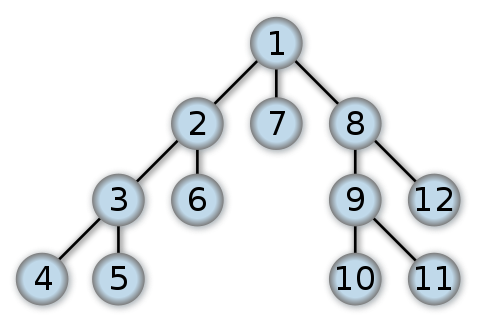
\includegraphics[width=0.3\textwidth]{img/dfs}
\end{center}

DFS can also be implemented with a recursive function:
instead of adding the neighbours to the waiting list, just calling the
visit procedure on them will have the same effect.
This may sound more simple, but internally it still uses the a stack,
the \emph{call stack}, that stores information about which functions
the program is in.

An interesting property is that the search never jumps from one side of the
graph to the other. After it has visited the first neighbour, the search only
has to go back to the original node through one edge,
then continue with the next neighbour.
In the above example, the path taken would be
$1,2,3,4,3,5,3,2,6,2,1,7,1,8,\ldots$
It goes through every edge exactly two times.

This makes it a viable option to physically traverse a graph (for example,
finding the center of a maze with loops, or exploring a cave system in
Minecraft) without having to remember anything, at the cost of a few markers.

\subsection{Breadth-first search}

\emph{Breadth-first search}, or \emph{BFS} uses a queue as a waiting list,
and that is literally the only difference in the implementation.

What changes is the order the nodes will be processed in.
Since the nodes are taken from the queue
in the same order as they were inserted,
the algorithm will first process all the neighbours of the starting point,
then when it has done that it will process the neighbours of the neighbours,
etc. It will work its way \emph{by layers}.

The diagram below shows the order in which nodes are visited for
the same example:
\begin{center}
    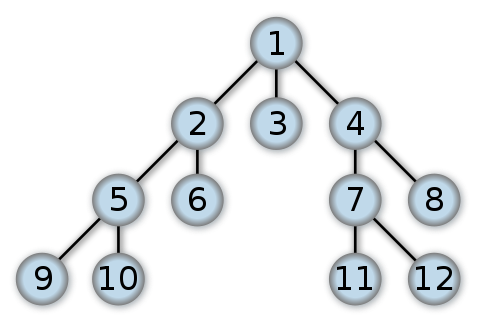
\includegraphics[width=0.3\textwidth]{img/bfs}
\end{center}

The advantage of BFS is that if we keep track of which edges it took
to get to the nodes, it gives us the shortest path from the starting point
to every node.
That is because of the order in which BFS visits the nodes.
It first makes sure all the nodes at distance 1 have been processed before
moving on to the nodes at distance 2, so we can be sure there was no path
shorter than 2. The same applies for distance 3, then 4, and so on.

Note that it only gives the shortest path in terms of number of edges.
If the edges have different costs (that is, if the graph is weighted),
then BFS will not work.

\subsection{Comparison}

Let $n$ be the number of nodes and $m$ the number of edges.
The complexity of both algorithms is $O(n+m)$,
assuming an adjacency list structure, so there is no time difference.
But this shows they are particularly efficient for sparse graphs.

As a consequence, the decision depends on their advantages.
DFS is simpler to implement if you use recursive functions,
and it is perfect if you cannot acess any node instantly.
BFS will mostly be useful when you have to find a shortest path
in a non-weighted graph.

